
\subsection{On walk bases for $\Delta$-modules for $l\geq 0$}
\label{ss:walkbases0}

We can go further than the combinatorial correspondence in (\ref{pr:walks0}). 
\ppm{[-can we actually?!  there is a lot of colour here.  might minimize this section for the first submission???]}

\mdef   Example. 
%\bajm{\sout{I have so far counted 13 walks of length 5 from $\emptyset$ to $(2,1)$, but in my calculation it has dim 14... I must be missing a walk...} got it!} 
Formally, 
%OK let's make a start on writing 
the walk-basis for 
$\Delta^{l=1}_{5,((21),0)}$    %in \bajm{( understood :) )}
is:
\begin{equation}  \label{eq:walkbasis521}
0-1-0-1-(2)-(21),
\;\;\; \;\;\; \hspace{.421cm}
0-1-0-1-(11)-(21),  \hspace{2.29762cm} 
\end{equation}
\[ 
0-1-(2)-1-(2)-(21),
\;\;\; \hspace{.31cm} 
0-1-(2)-1-(11)-(21),   \hspace{.53cm} 
\;
0-1-(11)-1-(2)-(21),
\] 
\[ 
0-1-(11)-1-(11)-(21),  \;\;\;
0-1-(2)-(21)-(2)-(21), \;\;\;
0-1-(2)-(21)-(11)-(21),
\]
\[ 
0-1-(2)-(21)-(21)'-(21), \hspace{1.9753185cm} 
0-1-(11)-(21)-(2)-(21), \hspace{.2cm} 
\]
\[ 
0-1-(11)-(21)-(11)-(21),  \;\;\; \hspace{1.95cm} 
0-1-(11)-(21)-(21)'-(21),
\]
\[ 
0-1-(2)-(3)-(2)-(21), \;\;\; \hspace{.96cm} 
0-1-(11)-(111)-(11)-(21)
\]

\mdef   \label{exa:l0p6la2}
Example. 
Explicit partial bases for  
$\Deltaa^{l=0,n=6}_{(4,(2))}$ is:  %and ... (not consistent with proper labelling \ppm{yet!}):  
\medskip 

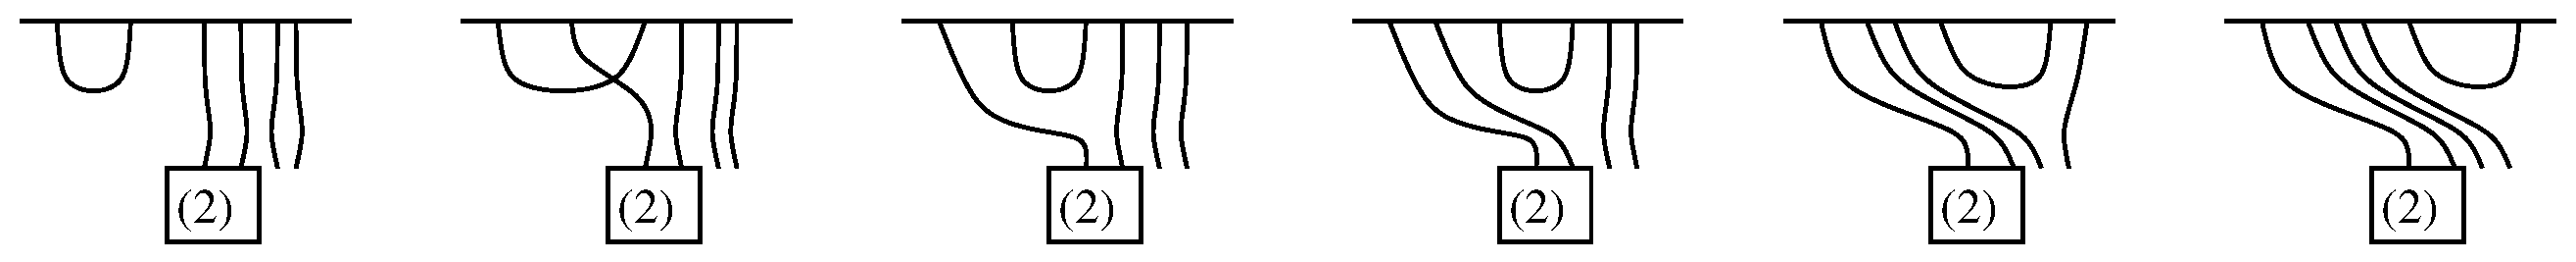
\includegraphics[width=10.9cm]{xfig-ppm/Delta62bas.eps}

\ppm{[So far the following is nonsense, but at least there are pics of diagrams. I'll fix it!...]}
The elements expressed as walks (writing $\lambda'''$ to mean $(\lambda,3)$ and so on):
\begin{align*}
    &0-1-0-1-(2)-(2)'-(2)''& &\sim e_{1,2}, \\
&0-1-(2)-1-(2)-(2)'-(2)'' &&\sim e_{2,3}, \\
&0-1-(11)-1-(2)-(2)'-(2)'' &&\sim e_{1,3}, \\
&0-1-(2)-(2)'-(2)-(2)'-(2)''&&\sim e_{3,4}, \\
&0-1-(2)-(2)'-(2)''-(2)'-(2)''&&\sim e_{4,5}, \\
& 0-1-(2)-(2)'-(2)''-(2)'''-(2)'' &&\sim e_{5,6},\end{align*}
(finish me!... \bajm{right? I am also suggesting the above correspondence with diagrams} \ppm{[-interesting. does that represent the application of an algorithm, or so far just a one-off?
For $l=-1$ of course the Rollet graph is just a simple chain $0-1-1'-1''-...$ which we could also label as $0-1-2-3-...$. There is a natural partial order on walks of length $n$ from 0 to (say) $s$, with $0-1-0-1-...-0-1-2-3-...-s$ the lowest and $0-1-2-...-max-...-(s+1)-s$ the highest. One can assign the diagram cup-cup-...-cup-line-line-...line to the lowest; and then construct the others iteratively so that if walk $w'$ is obtained from $w$ by $j-(j-1)-j \;\leadsto\; j-(j+1)-j$ (for some $j$) in position $i$ then the diagram $d'$ is given by $U_i d$. Does that make sense? (There is a more complicated version for Brauer. If we are lucky the general $l$ case (or at least some intermediate $l$ case) might be easy to interpolate.  - In which case this might even make the germ of a neat little paper.)]}\bajm{I think this represents the application of an algorithm which I don't quite understand yet :)... but seems quite accesible}). 


Aside. Here is another set of walks (for a different module! \bajm{for $\Delta^{l\geq 0}_{6,((2),0)}$ ?}):
\begin{align*} 
&0-1-0-1-0-1-(2), &&
0-1-0-1-(2)-1-(2),\\
&0-1-0-1-(11)-1-(2),
&&0-1-(2)-1-0-1-(2),
\\ &0-1-(2)-1-(2)-1-(2),
&&0-1-(2)-1-(11)-1-(2),
\\ &0-1-(11)-1-0-1-(2),
&&0-1-(11)-1-(2)-1-(2),
\\&0-1-(11)-1-(11)-1-(2).\end{align*}
(Is this correct?! \bajm{There should be more walks no? None of these walks go past $(2)$ in the rollet graph} \ppm{[-yes agreed. (I'm working in spurts as pain levels allow, so there'll be some mud in my tex-ing waters. hopefully more good than bad overall.  :-) )]})



\medskip  \noindent  Another example is
$\Delta^{l=1}_{4,(2)}$:  \medskip 

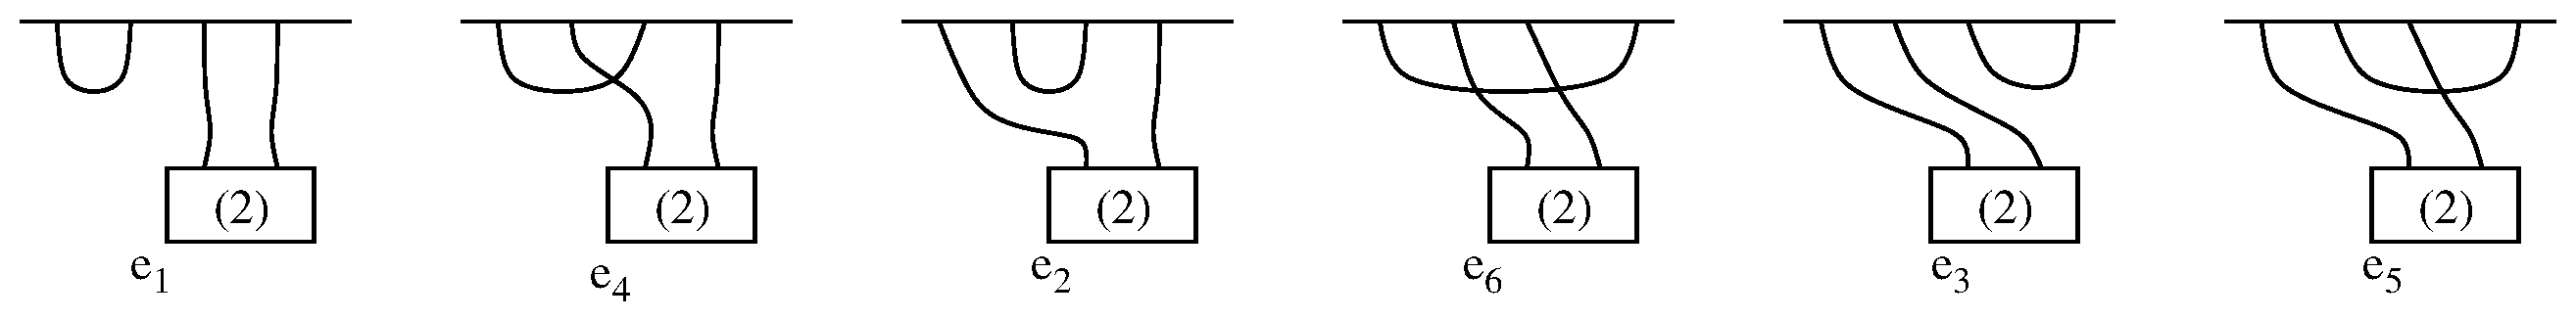
\includegraphics[width=10cm]{xfig-ppm/Delta42bas.eps}

The elements expressed as walks:  
\begin{align*}
    &0-1-0-1-(2), &&\sim e_{1,2}, &&0-1-(2)-1-(2),  &&\sim e_{2,3}, \\
&0-1-(2)-(3)-(2), &&\sim e_{3,4}, &&0-1-(2)-(21)-(2), &&\sim e_{2,4},\\
&0-1-(11)-1-(2), &&\sim e_{1,3}, &&0-1-(11)-(21)-(2), &&\sim e_{1,4}.
\end{align*}

\bajm{Next look at $\Delta^{l=1}_{6,((3),1)}$, $\Delta^{l=2}_{6,((4),0)}$... See if this sheds light on walk $\to$ diagram map:}
For $\Delta^{l=1}_{6,((3),1)}$, in addition to the walks included in the $l=0$ cases (now replacing $(2)^{'}$ with $(3)$, $(2)''$ with $(3)'$  etc) we also include:
\begin{align*}
    &0-1-(11)-(21)-(2)-(3)-(3)' &&\sim e_{1,4}, \\
&0-1-(2)-(21)-(2)-(3)-(3)'&&\sim e_{2,4},
\end{align*}

For $\Delta^{l=2}_{6,((2),2)}$ we include the previous walks (replacing $(3)'$ with $(4)$) and we include:
\begin{align*}
    &0-1-(11)-(21)-(31)-(3)-(4) &&\sim e_{1,5}, \\
&0-1-(2)-(21)-(31)-(3)-(4)&&\sim e_{2,5},\\
&0-1-(2)-(3)-(31)-(3)-(4)&&\sim e_{3,5},
\end{align*}
\bajm{I seem to be on the verge of being able to formulate a correspondence between walks and diagrams, at least in the case of 1D Specht-modules, by considering the positions of ``turnbacks" and ``deviations" from an ``ideal walk" (ideal walks i am tentatively defining as those which consist only of subdiagrams of the final diagram (need to modify to deal with going to right of final diagram...) ).   }


%
\section{Young Graph by Alcove Geometry}
This section is a small note, devoted to the idea of realising the Young Graph by alcove geometry. Firstly, consider the type $B_{\infty}$ Weyl group, $G$:
\[ G=\langle s_0, s_1,\dots \ | \ s_k^2=(s_0 s_1)^4=(s_{l}s_{l+1})^3=(s_i s_j)^2=e \ \text{for }l>0, |i-j|>1 \rangle,\]
acting on $\R^\infty$ (the space of finite real sequences) as follows:
\begin{align*}
    s_0(x_1,x_2,\dots,x_n)&=(-x_1,x_2,\dots,x_n),\\
    s_i(x_1,\dots,x_i,x_{i+1},\dots,x_n)&=(x_1,\dots,x_{i+1},x_i,\dots,x_n),
\end{align*}
where we use $(x_1,x_2,\dots,x_n)$ as short hand for the same infinite sequence, padded by 0s on the right. By allowing the $x_k$ to possibly be 0, we can ensure the last definition is always sensible. We can consider the $s_0$ as acting by reflection in the hyperplane defined by $x_1=0$, and the $s_i$ as acting by reflection in the hyperplane defined by $x_i=x_{i+1}$.

Given an element $(x)\in \R^\infty$ we can apply $s_0$ (conjugated by permutations to act in each component) so that all non-zero elements are positive, and then apply a permutation to order all entries in descending order. Thus a fundamental domain, $\mathcal{D}$, for $G\circlearrowright \R^\infty$, is the set of finite, descending, positive sequences:
\[\mathcal{D}= \left\{(x_1,x_2,\dots, x_n,0,\dots) \in \R^\infty \ \Bigg| \ \begin{matrix}\text{ for some } n\in \N \text{ such that }\\ x_1\geq x_2\geq \dots \geq x_n>0\end{matrix} \right\}.\]
Now, let us augment our group to be $\hat{G}$ where we add another generator $r_0$ to $G$ which satisfies the exact same relations as $r_0$ and has no ``braiding" relation with $s_0$. We give a Dynkin diagram for the group $\hat{G}$ below:
\[ \begin{tikzcd}[column sep=tiny,row sep = tiny]
    s_0\ar[dr,equal]\\
    &s_1\ar[r,dash]&s_2\ar[r,dash]&s_3\ar[r,dash]&\dots\\
    r_0\ar[ur,equal]\ar[uu,dash,"\infty"]
\end{tikzcd}\]
Now let $r_0$ act on $\R^\infty$ by the (affine) reflection in the hyperplane defined by $x_1=1$, that is,
\[r_0(x_1,x_2,\dots,x_n)=(2-x_1,x_2,\dots,x_n).\]
We then observe that $r_0 s_0$ acts by $x_1\mapsto x_1+2$ (fixing all other components). For a partition, $\l\vdash n$, we may view $\l=(\l_1,\l_2,\dots, \l_r)\in \mathcal{D}$ with $\l_i\geq \l_{i+1}$ for all $i$. Now define
\[\mathcal{D}_{\l}:=\{x\in \R^\infty \ | \ x-\l \in [0,1)^\infty  \}.\]
Clearly $\mathcal{D}=\sqcup_{\l} \mathcal{D}_{\l}$ and furthermore, we claim that each $\mathcal{D}_{\l}$ is a fundamental domain for $\hat{G}\circlearrowright \R^\infty$ (or an alcove) which shares a face with $\mathcal{D}_{\l'}$, if and only if, $\l'$ is a partition obtained from $\l$ by ``adding or removing a box". Suppose that $\l$ and $\l'=(\l_1,\dots,\l_i+1,\dots ,\l_r)$ are both partitions. Then $\mathcal{D}_{\l}$ and $\mathcal{D}_{\l'}$ (or rather, their closures) share the face
\[\overline{\mathcal{D}_{\l}}\cap\overline{\mathcal{D}_{\l'}}=\left\{\begin{matrix}(\l_1+\xi_1,\dots,\l_i+1,\dots,\l_r+\xi_r,\xi_{r+1},\dots,\xi_k)\in \mathcal{D}  \\ :\text{for some } k \in \N, \text{ where } \xi_l\in [0,1]\end{matrix} \right\}.\]
Therefore, by identifying each alcove $\mathcal{D}_{\l}$ with the underlying partition $\l$, we obtain the Young-graph as the dual graph of this alcove geometry.


   %% modularised into a file for ease of movement
%% ...and moved to the end of doc for now
